\documentclass[
twocolumn,
% hf,
]{ceurart}

% One can fix some overfulls
\sloppy

% Minted listings support 
% Need pygment <http://pygments.org/> <http://pypi.python.org/pypi/Pygments>
% \usepackage{minted}

% Add figures directory as graphics path
\graphicspath{ {./figures/} }

% Used for KL-divergence
\usepackage{mathtools}
\DeclarePairedDelimiterX{\infdivx}[2]{(}{)}{%
  #1\;\delimsize\|\;#2%
}
\newcommand{\infdiv}{D\infdivx}
\DeclarePairedDelimiter{\norm}{\lVert}{\rVert}

% Used for colored boxes in class legend table
\usepackage{tcolorbox}
% Custom column widths`
\usepackage{array}
\newcolumntype{N}{>{\centering\arraybackslash}m{.9cm}}
\newcolumntype{M}{>{\centering\arraybackslash}m{1.0cm}}
\newcolumntype{Z}{>{\centering\arraybackslash}m{1.6cm}}
\newcolumntype{Y}{>{\centering\arraybackslash}m{1.6cm}}
\usepackage{multirow}

% auto break lines
% \setminted{breaklines=true}

% end of the preamble, start of the body of the document source.
\begin{document}

% Rights management information.
% CC-BY is default license.
\copyrightyear{2021}
\copyrightclause{Copyright for this paper by its authors.
  Use permitted under Creative Commons License Attribution 4.0
  International (CC BY 4.0).}

% This command is for the conference information
\conference{Proceedings of the CIKM 2021 Workshops, November 1-5, Online}

% The "title" command
\title{Uncertainty-aware graph-based multimodal remote sensing}

% The "author" command and its associated commands are used to define
% the authors and their affiliations.
\author[1]{Iain~Rolland}[orcid=0000-0002-4137-5605, email=imr27@cam.ac.uk,]

\address[1]{Department of Engineering, University of Cambridge, Cambridge, CB2 1PZ United Kingdom}
\address[2]{Department of Physics and Technology, UiT the Arctic University of Norway, P.O. box 6050 Langnes, NO-9037, Tromsø, Norway}

\author[1,2]{Andrea~Marinoni}[orcid=0000-0001-6789-0915, email=andrea.marinoni@uit.no,]

\author[1]{Sivasakthy~Selvakumaran}[orcid=0000-0002-8591-0702,email=ss683@cam.ac.uk,]

% The abstract is a short summary of the work to be presented in the article.
\begin{abstract}
In order to adopt deep learning methods in environments where the decisions being made are high-stakes, it is important the methods are capable of quantifying the prediction confidence or uncertainty.
Graph-based convolutional neural networks can be trained to perform classification of multimodal remote sensing data using a model output which represents a Dirichlet distribution parameterization.
This parameterization can then also be used to obtain measures of prediction uncertainty.
By making a correspondence between a multinomial opinion, as described by subjective logic, and a Dirichlet distribution parameterization, a direct mapping between the two can be performed.
A multinomial opinion of this kind can produce quantified measures of uncertainty and distinguish uncertainty due to a lack of evidence (vacuity) and uncertainty due to conflicting evidence (dissonance).
With an appropriately chosen loss function, the graph-based classifier will converge to provide accurate estimates of uncertainty.
The results presented in this paper show that the measures of uncertainty provided by such models are capable of better distinguishing out-of-distribution data samples than probabilistic measures of uncertainty produced by equivalent deterministic neural networks.
\end{abstract}

% Keywords. The author(s) should pick words that accurately describe the work being presented. Separate the keywords with commas.
\begin{keywords}
  Multimodal remote sensing \sep
  uncertainty estimates \sep
  graph convolutional networks \sep
  subjective logic \sep
  land cover classification
\end{keywords}

% This command processes the author and affiliation and title information and builds the first part of the formatted document.
\maketitle

\section{Introduction}
The capability of algorithms to provide accurate measures of confidence and uncertainty is important if they are to be adopted in real-world scenarios where the stakes can be high \cite{Goodman2017}.
Although deep learning methods are often capable of producing high-accuracy predictions \cite{LeCun2015, LiangpeiZhang2016}, they are generally criticized for being unable to express when to have confidence in the prediction and when the prediction should be presented as uncertain.
If deep learning models are to be integrated reliably into real-world decision making processes, it is of vital importance that the methods being used are capable of accurately expressing uncertainty \cite{Lee2004}.

With remotely-sensed data being available with ever-greater temporal and spatial resolutions, the development of computational processing methods which are capable of robustly handling such large volumes of data will assist countless earth-monitoring applications \cite{Chi2016}.
Specifically, with data being captured now using a wide range of techniques with complementary strengths, the ability to combine this data into a multimodal analysis will allow each data mode to interact synergistically to provide better results than any individual data mode would produce in isolation.
Each data capturing technique will naturally have its own strengths and weaknesses, inherent to the physical properties of the sensing mode \cite{Chlaily2021, Marinoni2021}.
Deterministic classification, while useful, is held back by its inability to express uncertainty.
Adoption of such techniques will always be limited by the adopter's trust in the predictions.
Uncertainty estimates, however, will greatly assist human trust in models, as it will provide a quantification of confidence that might indicate when a prediction is not to be trusted, and more importantly, when a prediction is given with great certainty \cite{Chakraborty2017}.

In this paper, we have analyzed how well different measures of model uncertainty perform the task of identifying data points which belong from a distribution other than those observed during training (out of distribution detection).
To do so, we have used graph-based neural network architectures that are adapted to provide subjective opinions (as described in the field of belief or evidence theory \cite{Josang2018}) through the use of Dirichlet distribution parameterizations \cite{Kipf2017, ZhaoXujiang2020}.
Adopting such a method for performing multimodal classification of remote sensing data is, to the best of our knowledge, an as-yet untested approach.
The performance of the adopted technique represents a promising avenue in the search for meaningful uncertainty estimates when performing multimodal remote sensing classification.

The remainder of this paper is organized as follows: Section \ref{sec::unc_framework} describes the uncertainty framework adopted in the methods presented, Section \ref{sec::GraphNetworkArchitecture} details the construction of the graph-based neural networks used, Section \ref{sec::results} presents an analysis of results and Section \ref{sec::conclusion} summarizes and draws conclusions as well as suggests areas for future work.

\section{Uncertainty framework}
\label{sec::unc_framework}

% The framework described in this section is the same as is described by the work of \cite{ZhaoXujiang2020} where they use the approach to perform semi-supervised classification of benchmark graph classification datasets including Cora and Pubmed.
% The method they present has been adapted here to perform the task of multimodal remote sensing classification.

\subsection{Subjective Logic}
Subjective Logic (SL), takes an evidence-based approach to decision making \cite{Josang2016}.
Expressing an opinion using measured quantities of belief allows the distinction to be made between uncertainty due to a lack of evidence (vacuity) and uncertainty due to the presence of conflicting evidence (dissonance).
A multinomial opinion, $\omega$, can be expressed as $\omega=\left(\mathbf{b}, u, \mathbf{a}\right)$, where $\mathbf{b}$ is a belief mass vector, the scalar $u$ is the uncertainty mass and $\mathbf{a}$ is the base rate vector.
For a $K$-class classification problem, $\mathbf{y}$, $\mathbf{a}$ and $\mathbf{b}$ are all vectors of dimension $K$.
A projection of $\omega$ onto a probability distribution can be made according to
\begin{equation}
  P(y=k) = b_k + a_ku.
  \label{eq:prob_projection}
\end{equation}
It follows that since $\sum_{k=1}^Ka_k=1$ for the base rate vector, an additivity requirement is described by
\begin{equation}
    u+\sum_{k=1}^K b_k=1.
\end{equation}

\subsection{Dirichlet mapping}
If $\mathbf{p}$ is a $K$-dimensional random vector containing the probability of belonging to each output class, and $\boldsymbol{\alpha}$ is the strength vector which parameterizes a Dirichlet distribution, the probability density function of the Dirichlet is given by
\begin{equation}
    \textrm{Dir}(\mathbf{p}|\boldsymbol{\alpha})= \frac{\Gamma(\sum_{k=1}^K\alpha_k)}{\prod_{k=1}\alpha_k}\prod_{k=1}^Kp_k^{\alpha_k-1},
\end{equation}
where $\Gamma()$ is the gamma function.
The distribution's expected value is given by
\begin{equation}
\mathbb{E}\left[\textrm{Dir}(p_k\vert\boldsymbol{\alpha})\right]=\frac{\alpha_k}{\sum_{k=1}^K\alpha_k}.
\label{eq:expected_dir}
\end{equation}
If we allow the uncertainty mass and base rates to be given by
\begin{equation}
    u=\frac{K}{\sum_{k=1}^K\alpha_k}=\frac{K}{S}
\end{equation}
and
\begin{equation}
    a_k=1/K, \forall k
\end{equation}
respectively, where $S$ refers to the Dirichlet strength, then by equating the probability projection of (\ref{eq:prob_projection}) with the expected value of the Dirichlet distribution given by (\ref{eq:expected_dir}), the expression for the belief mass can be obtained as
\begin{equation}
    b_k = \frac{\alpha_k-1}{S}.
\end{equation}
This provides us with everything needed in order to map from a Dirichlet distribution to a SL opinion and vice versa.
\subsection{Uncertainty measures}
\label{sec::UncertaintyMeasures}
From the definitions of the evidential uncertainties presented in \cite{Josang2018}, the measures of vacuity and dissonance have been adopted.
The measure of vacuity uncertainty is simply given by the uncertainty mass, i.e.
\begin{equation}
    vac(\omega)\equiv u = \frac{K}{S},
\label{eq::vacuity}
\end{equation}
and the measure of dissonance uncertainty is given by
\begin{equation}
    diss(\omega)=\sum_{i=1}^K\left(\frac{b_i\sum_{j\neq i}b_j\textrm{Bal}(b_j,b_i)}{\sum_{j\neq i}b_j}\right),
\end{equation}
where $\textrm{Bal}()$ is a function which gives the relative balance between two belief masses, defined by
\begin{equation}
    \textrm{Bal}(b_j,b_i)=\begin{cases}1-\frac{\vert b_i-b_j\vert}{b_i+b_j},&\text{if } b_i+b_j\neq0,\\
    0,&\text{otherwise.}\end{cases}
\end{equation}

The differential entropy of the model predictions is also computed to provide a comparitive metric against which the evidential uncertainties can be compared.
% For a Bayesian model with inputs, outputs and parameters denoted $x$, $y$ and $\boldsymbol{\theta}$ respectively, the posterior, which will be approximated, is $p(\boldsymbol{\theta}\vert\mathcal{D})$, where $\mathcal{D}$ is the observed dataset.
% The total entropy, made up of both aleatoric and epistemic uncertainty \cite{Depeweg2018} is given by
% \begin{equation}
%     \mathcal{H}\left(\mathbb{E}_{p(\boldsymbol{\theta}\vert \mathcal{D})}\left[p(y\vert x;\boldsymbol{\theta}\right]\right),
% \end{equation}
% where $\mathcal{H}()$ computes the differential entropy of a distribution.
% Aleatoric uncertainty, which accounts for noise inherent to the data observations \cite{Kendall2017}, is given by
% \begin{equation}
%     \mathbb{E}_{p\left(\boldsymbol{\theta}\vert \mathcal{D}\right)}\left[\mathcal{H}(p(y\vert x; \boldsymbol{\theta}))\right].
% \end{equation}
% The epistemic uncertainty, therefore, is given by the difference between these two quantities
% \begin{equation}
%     \mathcal{H}\left(\mathbb{E}_{p(\boldsymbol{\theta}\vert \mathcal{D})}\left[p(y\vert x;\boldsymbol{\theta}\right]\right)-\mathbb{E}_{p\left(\boldsymbol{\theta}\vert \mathcal{D}\right)}\left[\mathcal{H}(p(y\vert x; \boldsymbol{\theta}))\right].
% \label{eq::epistemic}
% \end{equation}
% In order to compute the above expressions for aleatoric and epistemic uncertainty, the posterior distribution over models is approximated by samples obtained using dropout inference \cite{Gal2016}.

\section{Graph network architecture}
\label{sec::GraphNetworkArchitecture}
The multimodal data can be represented using a graph, where each of the $N$ nodes in the graph represents a pixel in the image.
The graph's adjacency matrix, $\mathbf{A}\in\mathbb{R}^{N\times N}$, is used to represent edges between nodes deemed similar.
A set of features, $\mathbf{X}\in\mathbb{R}^{N\times C}$, is used to assign a vector description of each graph node, where $C$ denotes the number of input features.
The graph's degree matrix, $\mathbf{D}\in\mathbb{R}^{N\times N}$, is a diagonal matrix with elements given by $\mathbf{D}_{ii}=\sum_j\mathbf{A}_{ij} $.

The graph convolutional networks (GCNs) used are of the form proposed by \cite{Kipf2017}, where the graph convolutional layer is given by
\begin{equation}
    \mathbf{Z}^{(l+1)}=\sigma\left(\tilde{\mathbf{D}}^{-\frac{1}{2}}\tilde{\mathbf{A}}\tilde{\mathbf{D}}^{-\frac{1}{2}}\mathbf{Z}^{(l)}\boldsymbol{W}^{(l)}\right),
\label{eq::gcn_layer}
\end{equation}
where $\mathbf{Z}^{(l)}$, $\mathbf{Z}^{(l+1)}$ and $\boldsymbol{W}^{(l)}$ are the inputs, outputs and weights of the $l^\textrm{th}$ layer respectively, and $\sigma()$ is a non-linear activation function.
For brevity, the tilde operator is used to represent the inclusion of self-connection edges in the graph, i.e. $\tilde{\mathbf{A}}=\mathbf{A}+\mathbf{I}$ and $\tilde{\mathbf{D}}=\mathbf{D}+\mathbf{I}$.

\subsection{Subjective models}
An adaptation to the GCN architecture used by \cite{Kipf2017} must be made in order to obtain subjective opinions that will be used to obtain measures of vacuity and dissonance uncertainty.
The adaptation made means that the model will output node-level Dirichlet distribution parameters, such that the output will provide a probability distribution over multinomial class probabilities for each node.
To do so, the softmax output activation function used in the output layer of the GCN is substituted for a ReLU function.
In this way, the model is trained to output non-negative evidence contributions, $\mathbf{E}\in\mathbb{R}^{N\times K}$, where $\mathbf{E}_{i} = \boldsymbol{\alpha}_{i}-\mathbf{1}$ and $\boldsymbol{\alpha}_{i}$ refers to the $K$-dimensional concentration parameters of the $i^\text{th}$ node.
In order to train such a model, the loss function is made up of two components: a squared error term, which is minimized in order to classify a greater proportion of the nodes correctly, and a variance term, which is minimized to incentivize the model to provide confident predictions where possible.
This loss, $\mathcal{L}(\boldsymbol{\theta})$, is given by
\begin{equation}
\begin{split}
    \mathcal{L}(\boldsymbol{\theta})=\sum_{i\in\mathbb{L}}\sum_k \left[(p_{ik}-y_{ik})^2+\text{Var}(p_{ik})\right],\\
    =\sum_{i\in\mathbb{L}}\sum_k \left[(p_{ik}-y_{ik})^2+\frac{\alpha_{ik}}{S_i^2}\left(\frac{S_i-\alpha_{ik}}{S_i-K}\right)\right],
\end{split}
\label{eq:core_loss}
\end{equation}
where $i\in\mathbb{L}$ refers to the fact that the loss is computed using a sum only over nodes in the training set, $\mathbb{L}$.
Models trained with such an output activation and loss function will be denoted using the `S-' prefix in order to indicate they provide subjective predictions, e.g. S-GCN.

\subsection{Convergence assistance techniques}
In order to assist the convergence of subjective models, two additional assistance techniques have been used: teacher knowledge distillation and the use of a Dirichlet prior.
These have been shown to allow subjective models to provide better uncertainty estimates \cite{ZhaoXujiang2020}.
\subsubsection{Teacher knowledge distillation}
By training a non-subjective model in advance, its outputs, $\hat{p}_{ik}$, can be used in order to encourage the subjective model to converge to node Dirichlet distributions with $\mathbb{E}[p_{ik}]$ which are close to the teacher's deterministic estimates.
This is achieved using an additional term in the loss function,
\begin{equation}
    \mathcal{L}_{\text{T}}(\boldsymbol{\theta})=\sum_i\sum_k\left(\hat{p}_{ik}\log\frac{\hat{p}_{ik}}{\mathbb{E}[p_{ik}]}\right),
\end{equation}
which corresponds to the summation of KL-divergence terms between the teacher output probability and the expected value of the subjective model's Dirichlet distribution for each node, $\sum_i\infdiv{\hat{p}_{ik}}{\mathbb{E}[p_{ik}]}$.
Notice that this sum is computed over all nodes as opposed to just the nodes in $\mathbb{L}$.
Models trained using a teacher are denoted using the ``-T'' suffix e.g. a S-BGCN-T model would indicate that a pre-trained GCN was used as a teacher in order to assist the training convergence of a subjective graph convolutional model.
\subsubsection{Dirichlet prior}
A second convergence assistance technique which can be used involves the use of a Dirichlet prior, $\hat{\boldsymbol{\alpha}}$.
The exact method chosen to provide $\hat{\boldsymbol{\alpha}}$ will depend on the nature of the problem but we will assume nodes which are nearby in the graph are more likely to belong to the same output class than nodes which are far apart, a property known as homophily \cite{HuangQian2019}.
Using this assumption, we can use the computed distances on the graph to assign contributions of evidence from observed node labels to the other nodes in the graph using a function of our choosing.
If $d_{ij}$ denotes the shortest path distance between a given node, indexed by $i$ and an observed node, indexed by $j$, then the amount of evidence contributed to suggest that the $i^\text{th}$ node belongs to the $k^\text{th}$ class is given by
\begin{equation}
    h_{ik}(y_j,d_{ij})=
    \begin{cases}
      \frac{\exp{\left(\frac{-d_{ij}^2}{2\sigma^2}\right)}}{\left(2\pi\sigma^2\right)^{1/2}}, & \text{if } y_{jk}=1,\\
    0, & \text{otherwise},
    \end{cases}
\end{equation}
where $\sigma$ is a scale parameter which controls the order of distance magnitude over which evidence will propagate in the prior.
The total evidence to suggest the $i^\text{th}$ node belongs to the $k^\text{th}$ class, $e_{ik}$ can be found by summing these contributions over the nodes in the training set, such that the element in the prior is given by 
\begin{equation}
    \hat{\boldsymbol{\alpha}}_{ik}=1+e_{ik}=1+\sum_{j\in\mathbb{L}}h_{ik}(y_j, d_{ij}).
\end{equation}
The KL-divergence between the Dirichlet distribution of the prior and the model output is given by the term
\begin{equation}
    \mathcal{L}_{\text{K}}(\boldsymbol{\theta})=\sum_i\infdiv{\text{Dir}(\mathbf{p}_i\vert\boldsymbol{\alpha}_i)}{\text{Dir}(\hat{\mathbf{p}}_i\vert\hat{\boldsymbol{\alpha}}_i)},
\label{eq::teacher_loss}
\end{equation}
which can, in turn, be incorporated into the total loss function.
Models trained using a prior are denoted using the ``-K'' suffix.

Table \ref{loss_table} shows how these convergence assistance techniques can be weighted and combined in various permutations to provide a total loss function, $\mathcal{L}_\text{total}(\boldsymbol{\theta})$, as well as the model name abbreviations used to denote which combination has been used.
The "B" in the model names of Table \ref{loss_table} refers to the fact that dropout inference has been used as a Bayesian approximation, as mentioned in Section \ref{sec::UncertaintyMeasures}.
The coefficients $\lambda_{\text{T}}$ and $\lambda_{\text{K}}$ are used to control the relative importance of the teacher network and the Dirichlet prior respectively against the importance of the subjective loss function given in (\ref{eq:core_loss}).
These have been considered as hyperparameters which are to be tuned during training.

\begin{table}[!t]
\scriptsize
\renewcommand{\arraystretch}{1.5}
\caption{Loss function components and their weighting coefficients for different model types}
\label{loss_table}
\centering
\begin{tabular}{cc}
\hline
\bfseries Model name & \bfseries $\mathcal{L}_{\text{total}}(\boldsymbol{\theta})$\\
\hline
S-BGCN & $\mathcal{L}(\boldsymbol{\theta})$ \\
S-BGCN-T & $\mathcal{L}(\boldsymbol{\theta})+\lambda_{\text{T}}\mathcal{L}_{\text{T}}(\boldsymbol{\theta})$ \\
S-BGCN-K & $\mathcal{L}(\boldsymbol{\theta})+\lambda_{\text{K}}\mathcal{L}_{\text{K}}(\boldsymbol{\theta})$ \\
S-BGCN-T-K & $\mathcal{L}(\boldsymbol{\theta})+\lambda_{\text{T}}\mathcal{L}_{\text{T}}(\boldsymbol{\theta})+\lambda_{\text{K}}\mathcal{L}_{\text{K}}(\boldsymbol{\theta})$ \\
\hline
\end{tabular}
\end{table}

\section{Results and analysis}
\label{sec::results}
\subsection{Data}
A subsection of the 2018 IEEE GRSS Data Fusion Challenge dataset was selected for the purposes of validating the described methods.
The ground truth labels in this dataset describe 20 different urban land cover/land use classes (i.e. $K=20$) as well as an unlabelled state, described as Unclassified.
The modes of input data represent measurements from three sensor types: LiDAR, optical and hyperspectral (HS).
The LiDAR data was provided at $0.5$ m resolution, the same resolution as the ground truth labels (GT).
In order to simplify analysis, the optical data (which was provided at $0.05$ m resolution) and the HS data (which was provided at $1.0$ m resolution) were bilinearly resampled to obtain $0.5$ m resolution across inputs and outputs.

The graph was constructed with each $0.5$ m $\times$ $0.5$ m pixel representing a node in the graph.
Each node has a 52-dimensional feature vector describing it (produced by stacking 3 optical channels, 48 HS channels and 1 LiDAR channel).
The graph edges are computed using a $k$-nearest neighbors algorithm with two nodes receiving an edge connecting them if either node was one of the $k$ nodes which were nearest the other.
This produces a graph which is both undirected and unweighted.
The graph, which contains approximately 2.16 million nodes, was computed with $k=15$.

In order to measure an uncertainty output's ability to separate OOD nodes, a receiver operating characteristic (ROC) curve and a precision-recall (PR) curve can be computed.
The area under the ROC curve and PR curve (AUROC and AUPR respectively) can be used as a single numerical representation of the detection performance, where an area of $1.0$ would represent a perfect discriminator for both metrics.

% The exact types and abundances of these classes can be found in Table \ref{tab::classes}.
% The classes which do not appear in the subsection of the dataset but exist within the wider GT are included for completeness.

% \begin{table}
% % \renewcommand{\arraystretch}{1.5}
% \caption{Land cover/Land use classes in selected subsection of Houston dataset ground truth}
% \label{tab::classes}
% \centering
% \begin{tabular}{NNcZ}
% \hline
% \bfseries Class Value & \bfseries Legend Color & \bfseries Class Name & \bfseries Number of Nodes (total)\\
% \hline
% $0$ & \colorbox[rgb]{0.0,0.0,0.0}{\textcolor{white}{\phantom{A}}} & Unclassified & $1302595$\\
% $1$ & \colorbox[rgb]{0.0,1.0,0.03}{\textcolor{white}{\phantom{A}}} & Healthy grass & $10120$ \\
% $2$ & \colorbox[rgb]{0.21, 0.69, 0.15}{\textcolor{white}{\phantom{A}}} & Stressed grass & $16332$ \\
% $3$ & \colorbox[rgb]{0.53, 0.73, 0.57}{\textcolor{white}{\phantom{A}}} & Artificial turf & $0$ \\
% $4$ & \colorbox[rgb]{0.  , 0.47, 0.08}{\textcolor{white}{\phantom{A}}} & Evergreen trees & $38288$ \\
% $5$ & \colorbox[rgb]{0.  , 0.3 , 0.}{\textcolor{white}{\phantom{A}}} & Deciduous trees & $3082$ \\
% $6$ & \colorbox[rgb]{0.75, 0.48, 0.08}{\textcolor{white}{\phantom{A}}} & Bare earth & $0$ \\
% $7$ & \colorbox[rgb]{0.  , 0.89, 0.89}{\textcolor{white}{\phantom{A}}} & Water & $332$ \\
% $8$ & \colorbox[rgb]{0.98, 0.98, 0.98}{\textcolor{white}{\phantom{A}}} & Residential buildings & $12417$ \\
% $9$ & \colorbox[rgb]{0.94, 0.76, 0.92}{\textcolor{white}{\phantom{A}}} & Non-residential buildings & $587141$ \\
% $10$ & \colorbox[rgb]{1.  , 0.35, 0.36}{\textcolor{white}{\phantom{A}}} & Roads & $68831$ \\
% $11$ & \colorbox[rgb]{0.64, 0.64, 0.64}{\textcolor{white}{\phantom{A}}} & Sidewalks & $96020$ \\
% $12$ & \colorbox[rgb]{0.36, 0.36, 0.36}{\textcolor{white}{\phantom{A}}} & Crosswalks & $3584$ \\
% $13$ & \colorbox[rgb]{0.79, 0.  , 0.01}{\textcolor{white}{\phantom{A}}} & Major thoroughfares & $17181$ \\
% $14$ & \colorbox[rgb]{0.54, 0.  , 0.04}{\textcolor{white}{\phantom{A}}} & Highways & $0$ \\
% $15$ & \colorbox[rgb]{1.  , 0.65, 0.07}{\textcolor{white}{\phantom{A}}} & Railways & $0$ \\
% $16$ & \colorbox[rgb]{1.,1.,0.}{\textcolor{white}{\phantom{A}}} & Paved parking lots & $7677$ \\
% $17$ & \colorbox[rgb]{0.92, 0.44, 0.}{\textcolor{white}{\phantom{A}}} & Unpaved parking lots & $0$ \\
% $18$ & \colorbox[rgb]{0.98, 0.  , 1.}{\textcolor{white}{\phantom{A}}} & Cars & $0$ \\
% $19$ & \colorbox[rgb]{0.  , 0.  , 1.}{\textcolor{white}{\phantom{A}}} & Trains & $0$ \\
% $20$ & \colorbox[rgb]{0.49, 0.76, 0.8}{\textcolor{white}{\phantom{A}}} & Stadium seats & $0$ \\
% \hline
% \end{tabular}
% \end{table}

\begin{figure}[!t]
\centering
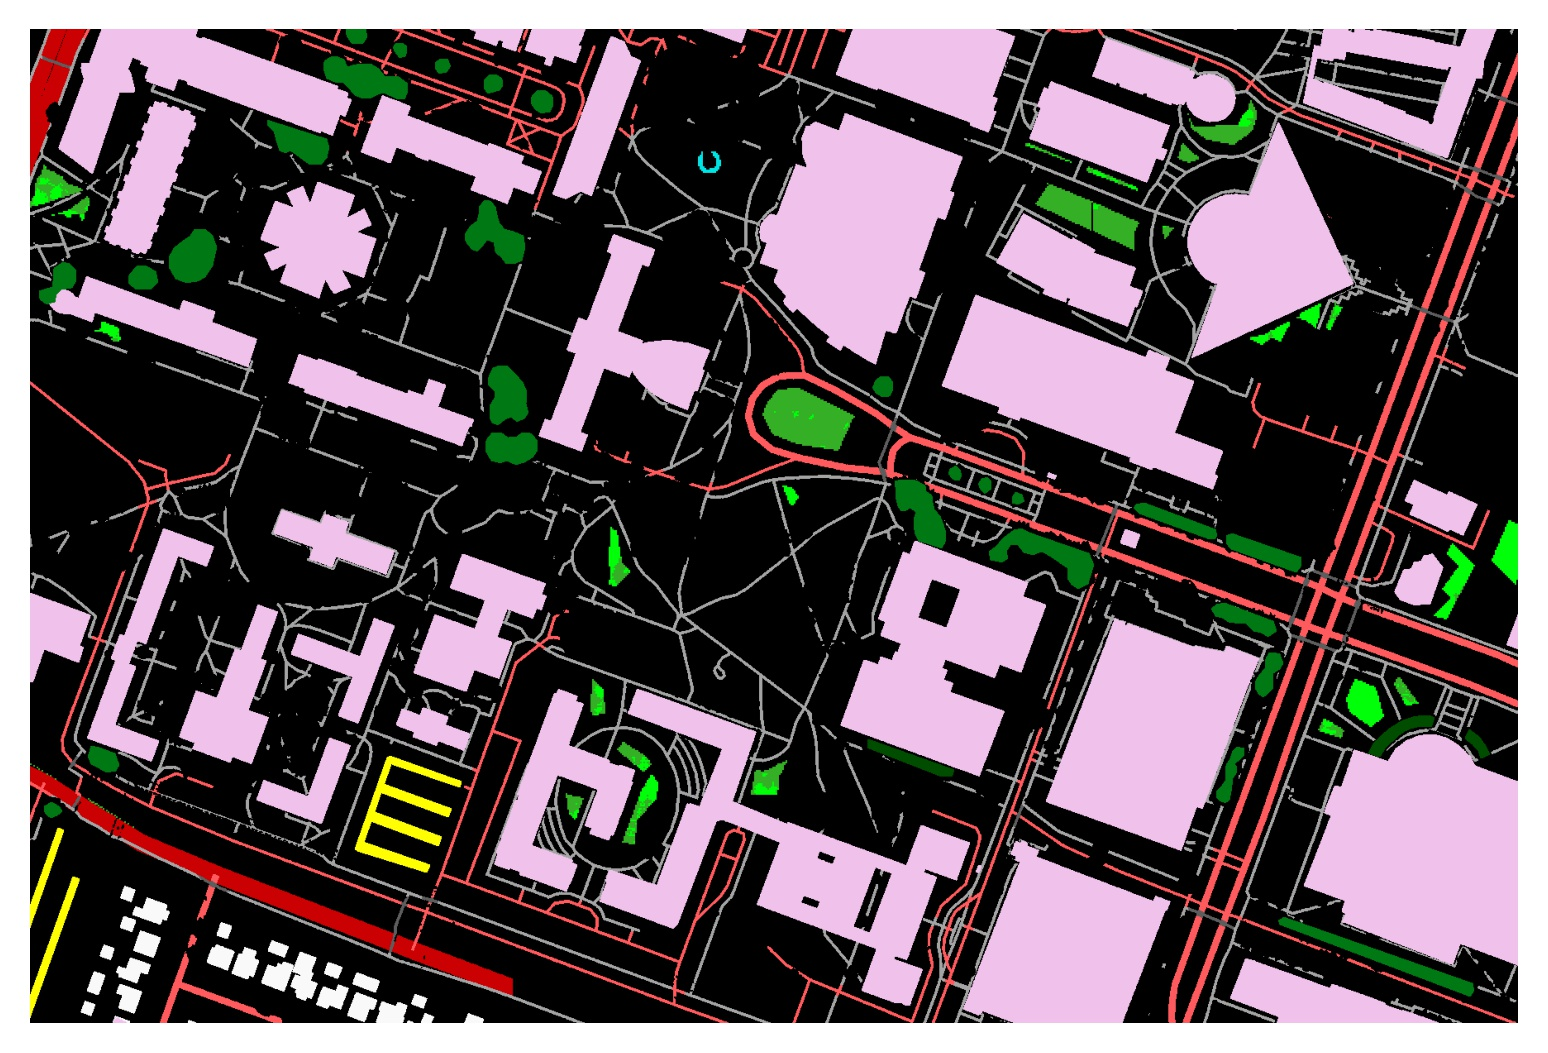
\includegraphics[width=.7\columnwidth]{figures/gt.jpg}
\caption{Ground truth data with colors depicting land cover classes. This data represents a subset of the 2018 IEEE GRSS Data Fusion Challenge dataset.}
\label{fig::gt}
\end{figure}

% In order to divide the annotations into a training, a validation and a test set, any adjacent pixels with the same label were considered part of one contiguous label block.
% Before randomly allocating these contiguous label blocks into the different sets, the blocks were separated along grid lines in order to prevent any prevent large contiguous blocks from skewing class balances between sets (see Figure \ref{fig::dataset_split} for a depiction of a random split).
% The resulting set of blocks were then randomly allocated into training, validation and test sets with proportions of 40\%, 30\% and 30\% respectively.
% This method of assigning contiguous blocks into a split together as opposed to randomly splitting pixels was done so as to reduce the number of strongly correlated samples (due to local spatial correlations in the input vectors) across the test/validation/test sets which would come with having pixels of immediate proximity split into different sets.
% 
% \begin{figure}[!t]
% \centering
% 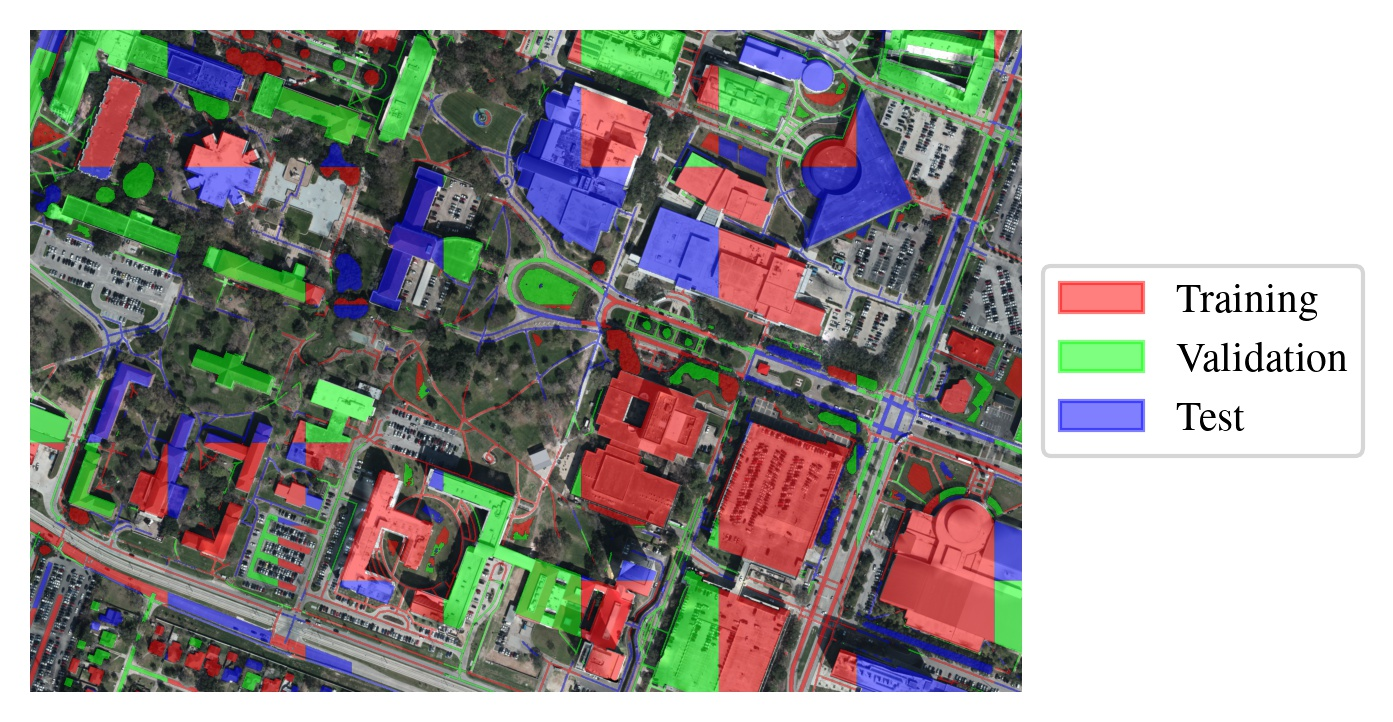
\includegraphics[width=\columnwidth]{figures/dataset_split.jpg}
% \caption{RGB data channels with overlaying colors used to depict a random dataset split with the red, green and blue overlay colors representing training, validation and test set pixels respectively.}
% \label{fig::dataset_split}
% \end{figure}

\subsection{Network training and hyperparameters}
Models were implemented and trained using the TensorFlow library \cite{Abadi2015}.
In order to handle the imbalance of classes in the dataset, sample weighting was used.
Samples were given weights which were inversely proportional to the number of total samples of each class in the training set.
This allows the losses related to nodes from under-represented classes to have an increased influence over parameter updates and vice versa.

All GCN-based models were constructed using a dropout layer (dropout probability $0.5$), a graph convolutional layer, as described in (\ref{eq::gcn_layer}), a second dropout layer (dropout probability $0.5$) and a second graph convolutional layer with the relevant output activation function.
The kernel weights of the first graph convolutional layer were regularized using an $L_2$ penalization.
Where dropout inference has been used, the number of samples taken was 100.

Hyperparameters including the learning rate, the $L_2$ regularization coefficient and the number of GCN layer output features, $F$, were selected via a grid-search method.
Where used, $\lambda_{\text{T}}$ and $\lambda_{\text{K}}$ were also found using a grid-search.

Learning was performed for a maximum of 400 epochs, but was stopped early if the validation loss failed to decrease further for 60 consecutive epochs.
If stopped early, model weights were returned to the settings which provided the lowest validation set loss upon the termination of training.

Each test was performed for different random dataset splits and model weight initializations to obtain mean and standard deviation measures of performance.

A benchmark has been provided by training `standard' GCNs which provide prediction entropy as a form of uncertainty estimate.

% \begin{table*}[!t]
% \renewcommand{\arraystretch}{1.3}
% \caption{Misclassification detection: Ability of each uncertainty type to detect misclassifications (measured by AUROC and AUPR).}
% \label{tab::misc_auroc}
% \scriptsize
% \begin{center}
% \begin{tabular}{Y|ccccc|ccccc}
% \hline
% \multirow{2}{*}{Model}  & \multicolumn{5}{c}{AUROC}\vline&\multicolumn{5}{c}{AUPR}        \\
%                         & Vac. & Dis. & Ale. & Epi. & Ent. & Vac. & Dis. & Ale. & Epi. & Ent. \\ \hline 
% % S-BGCN-T-K (superpixel prior) & $0.676$ & $0.801$ &$0.792$&$0.509$&$0.798$&$0.352$&$0.398$&$0.467$&$0.237$&$0.474$    \\
% S-BGCN-T-K  & $0.908$ & $0.840$ &$0.905$&$0.451$&$\mathbf{0.912}$&$0.659$&$0.545$&$0.649$&$0.206$&$\mathbf{0.672}$  \\
% S-BGCN-T & $0.729$ & $0.834$ &$0.869$&$0.618$&$0.861$&$0.451$&$0.484$&$0.591$&$0.278$&$0.579$  \\ 
% S-BGCN & $0.760$ & $0.877$ &$0.894$&$0.623$&$0.886$&$0.489$&$0.558$&$0.633$&$0.268$&$0.616$  \\ 
% S-GCN & $0.729$ & $0.842$ &-&-&$0.859$&$0.472$&$0.538$&-&-&$0.595$  \\ 
% S-MLP &$0.845$&$0.904$&-&-&$0.909$&$0.417$&$0.566$&-&-&$0.606$  \\
% GCN & - & - &-&-&$0.887$&-&-&-&-&$0.606$  \\ 
% Drop-GCN & - & - &$0.897$&$0.552$&$0.887$&-&-&$0.619$&$0.243$&$0.600$  \\ \hline
% \end{tabular}
% \end{center}
% \end{table*}

% \subsection{Misclassification detection}
% 
% Given that model uncertainties should provide a measure of the confidence which can be had about a model's predictions, a worthwhile estimate of uncertainty should be able to distinguish model misclassifications from accurate classifications.
% 
% 
% Models of each type described (as well as benchmark models) were trained and their outputs analyzed to produce the AUROC and AUPR values seen in Table \ref{tab::misc_auroc}.
% 
% % \begin{table*}[!t]
% % \renewcommand{\arraystretch}{1.3}
% % \caption{Misclassification detection: Ability of each uncertainty type to detect misclassifications (measured by the AUPR metric).}
% % \label{tab::misc_aupr}
% % \scriptsize
% % \begin{center}
% % \begin{tabular}{cccccc}
% % \hline
% % \multirow{2}{*}{Model}  & \multicolumn{5}{c}{AUPR}             \\
% %       & Vac. & Dis. & Ale. & Epi. & Ent. \\ \hline 
% % S-BGCN-T-K (superpixel prior) & $0.352$&$0.398$&$0.467$&$0.237$&$0.474$ \\
% % S-BGCN-T-K (pixel prior) & $0.659$&$0.545$&$0.649$&$0.206$&$\mathbf{0.672}$ \\
% % S-BGCN-T & $0.451$&$0.484$&$0.591$&$0.278$&$0.579$ \\ 
% % S-BGCN & $0.489$ & $0.558$  &$0.633$&$0.268$&$0.616$ \\ 
% % S-GCN & $0.472$ & $0.538$  &-&-&$0.595$ \\ 
% % S-MLP & $0.417$&$0.566$&-&-&$0.616$ \\
% % GCN & - & -  &-&-&$0.606$ \\ 
% % Drop-GCN & - & -  & $0.619$&$0.243$&$0.600$ \\ \hline
% % \end{tabular}
% % \end{center}
% % \end{table*}
% 
% The S-BGCN-T-K model achieves the best misclassification detection performance, with the uncertainty measured by entropy providing the best distinguishing metric, with AUROC and AUPR of $0.912$ and $0.672$ respectively, closely followed by the performance achieved by the measures of vacuity (AUROC and AUPR of $0.908$ and $0.659$ respectively) and aleatoric uncertainty (AUROC and AUPR of $0.905$ and $0.649$ respectively).

\subsection{Out of distribution detection}

It would also be reasonable to expect that uncertainty should be higher when the model is asked to make a prediction using an input which does not resemble the inputs upon which it was trained.
The relative inability of neural networks to successfully extrapolate beyond the support of the training data is a well-known weakness of these methods \cite{Lakshminarayanan2017}.
By training models using only a subset of the classes provided by the GT, with the other classes acting as out of distribution (OOD) samples, the OOD detection ability of the uncertainty metrics can be measured.
The AUROC and AUPR can be calculated for each uncertainty output provided by each model type, in order to determine the relative performance of the respective metrics for this task.

In the results presented, two classes were randomly selected to act as OOD.
This was repeated 10 times, with two new randomly sampled classes selected for each training and evaluation loop in order that the variation in OOD detection performance due to the nature of the classes selected as OOD could be averaged out and the mean and standard deviation computed.
Each model type was assessed over the same 10 sampled OOD class pairs for fairness.
The AUROC and AUPR values measured can be found in Table \ref{tab::ood}.

\begin{table*}[!t]
\renewcommand{\arraystretch}{1.3}
\caption{OOD detection: Ability of each uncertainty type to detect OOD nodes (measured by the AUROC and AUPR metrics). Values shown represent the mean $\pm$ standard deviation.}
\label{tab::ood}
\scriptsize
\begin{center}
\begin{tabular}{Y|ccc|ccc}
\hline
\multirow{2}{*}{Model}  & \multicolumn{3}{c|}{AUROC} & \multicolumn{3}{c}{AUPR} \\
                        & Vacuity & Dissonance & Entropy & Vacuity & Dissonance & Entropy\\ \hline 
% S-BGCN-T-K (superpixel prior) & $0.839\pm0.092$ & $0.691\pm0.173$ &$0.831\pm0.079$&$0.268\pm0.180$&$0.833\pm0.076$    \\           
S-BGCN-T-K & $\mathbf{0.882\pm0.085}$ & $0.605\pm0.197$ & $0.878\pm0.089$ & $\mathbf{0.318\pm0.289}$ & $0.132\pm0.184$ & $0.316\pm0.306$  \\        
S-BGCN-T & $0.588\pm0.147$ & $0.664\pm0.133$ & $0.578\pm0.186$ & $0.128\pm0.187$ & $0.137\pm0.192$ & $0.143\pm0.208$   \\ 
S-BGCN & $0.586\pm0.147$ & $0.666\pm0.132$ & $0.580\pm0.191$ & $0.127\pm0.186$ & $0.139\pm0.190$ & $0.145\pm0.209$  \\ 
S-GCN & $0.580\pm0.145$ & $0.650\pm0.120$ & $0.586\pm0.181 $ & $0.125\pm0.185$ & $0.130\pm0.191$ & $0.143\pm0.207$   \\ 
S-MLP & $0.767\pm0.152$ & $0.805\pm0.114$ & $0.787\pm0.125$ & $0.245\pm0.214$ & $0.233\pm0.170$ & $0.219\pm0.201$   \\   
GCN & - & - & $0.538\pm0.188$ & - & - & $0.116\pm0.179$  \\  \hline
% Drop-GCN & - & - & $0.538\pm0.187$ & - & - & $0.116\pm0.179$  \\ \hline
\end{tabular}
\end{center}
\end{table*}

% \begin{table*}[!t]
% \renewcommand{\arraystretch}{1.3}
% \caption{OOD detection: Ability of each uncertainty type to detect OOD nodes (measured by the AUPR metric). Values shown represent the mean $\pm$ standard deviation.}
% \label{tab::ood_aupr}
% \scriptsize
% \begin{center}
% \begin{tabular}{Y|ccccc}
% \hline
% \multirow{2}{*}{Model}  & \multicolumn{5}{c}{AUPR}             \\
%       & Vacuity & Dissonance & Aleatoric & Epistemic & Entropy \\ \hline 
% % S-BGCN-T-K (superpixel prior) &$0.234\pm0.252$&$0.142\pm0.185$&$0.214\pm0.249$&$0.099\pm0.227$&$0.212\pm0.251$    \\   
% S-BGCN-T-K &$\mathbf{0.318\pm0.289}$&$0.132\pm0.184$&$0.316\pm0.306$&$0.082\pm0.178$&$0.316\pm0.306$    \\        
% S-BGCN-T &$0.128\pm0.187$&$0.137\pm0.192$&$0.148\pm0.211$&$0.095\pm0.193$&$0.143\pm0.208$    \\ 
% S-BGCN & $0.127\pm0.186$ & $0.139\pm0.190$  &$0.150\pm0.213$&$0.095\pm0.195$&$0.145\pm0.209$    \\ 
% S-GCN & $0.125\pm0.185$ & $0.130\pm0.191$  &-&-&$0.143\pm0.207$    \\ 
% S-MLP & $0.245\pm0.214$ & $0.233\pm0.170$ &-&-&$0.219\pm0.201$    \\   
% GCN & - & -  &-&-&$0.116\pm0.179$    \\ 
% Drop-GCN & - & -  & $0.116\pm0.179$&$0.115\pm0.257$&$0.116\pm0.179$    \\ \hline
% \end{tabular}
% \end{center}
% \end{table*}

For the task of OOD detection, the S-BGCN-T-K model is the highest ranked model.
Its measure of vacuity uncertainty provided the best distinguishing metric, with mean AUROC and AUPR of $0.882$ and $0.318$ respectively, closely followed by performance from the measure of entropy (AUROC and AUPR of $0.878$ and $0.316$ respectively).
The performance of the S-BGCN-T-K model stands out above the performance of other models trained.
This highlights the importance of the convergence assistance techniques used, particularly the use of a meaningful prior.

The fact that vacuity is the uncertainty measure which best distinguishes OOD nodes reflects intuition.
Since vacuity measures the absence of evidence for a prediction, it is natural to expect that it would better distinguish OOD nodes for which the model ought to have little evidence to support its predictions.

\section{Conclusion}
\label{sec::conclusion}

In this paper we have adapted a novel classification method capable of providing uncertainty estimates to the task of multi-class classification of multimodal remote sensing data.
The adopted framework, based upon the theory of Subjective Logic, provides measures of vacuity and dissonance which are better capable of identifying out of distribution samples than the alternative probabilistic measures of uncertainty assessed.
Experimental results have shown the performance of the S-BGCN-T-K model for OOD detection to be improved against baseline methods.
This represents a promising avenue for uncertainty-aware learning in the task of multimodal remote sensing classification.

The presented results illustrate the importance of convergence assistance techniques as a means for improving the quality of uncertainty estimates, particularly through the use of a prior.
This can be seen by comparing the S-BGCN-T-K OOD detection performance with equivalent models which do not use a prior, e.g. S-BGCN-T.
% Of the uncertainty measures produced by the S-BGCN-T-K model, the measures of vacuity, aleatoric uncertainty or entropy all provide near-best performance for the identifying misclassifications.
In order to identify OOD nodes, the measure of vacuity stands out as the best-performing uncertainty metric.

Future work should consider the generalisation potential of this method by assessing performance on other challenging remote sensing classification datasets.
There is also scope for research into how the choice of method for computing the $\hat{\boldsymbol{\alpha}}$ prior affects the quality of uncertainty estimates, either by varying the scale parameter, $\sigma$, or considering different prior computation methods entirely.
% The acknowledgments section is defined using the "acknowledgments" environment
% (and NOT an unnumbered section). This ensures the proper
% identification of the section in the article metadata, and the
% consistent spelling of the heading.
\begin{acknowledgments}
This work is funded in part by Centre for Integrated Remote Sensing and Forecasting for Arctic Operations (CIRFA) and the Research Council of Norway (RCN Grant no. 237906), the Automatic Multisensor remote sensing for Sea Ice Characterization (AMUSIC) Framsenteret ``Polhavet'' flagship project 2020, the Isaac Newton Trust, and Newnham College, Cambridge, UK.
\end{acknowledgments}

% Define the bibliography file to be used
\bibliography{bibtex/bib/IEEEabrv, bibtex/bib/imrolland}

\end{document}
